\section{高速化に対する球密度の影響}
\label{sec:density}
超音波照射による擬塑性流体中の落下球の高速化に対する,球密度の影響を調べる.実験条件をTable\ref{table:exp-conditions}に示す.式(\ref{eq:Udiff})より,落下球高速化は球径の影響を受けることが示唆される.しかし本実験条件では,球径の差が5\%程度にとどまることから,密度変化による影響のみに注目し,球径は同一として考える.

実験によって得た落下速度の時間変化をFig\ref{fig:0.05-0.2}-\ref{fig:1.5}に示す.これより求めた,超音波照射のない状態の終端速度$U_\text{off}$と密度差$\Delta\rho$の関係をFig\ref{fig:rhoUT}に示す.当然ながら,密度差が大きくなると,終端速度が大きくなる.超音波照射のない落下速度の理論式(\ref{eq:UT})より,密度差のべき乗として,終端速度は以下の比例関係が成り立つ.
\begin{eqnarray}
    U_\text{off}\sim \left(\Delta\rho\right)^{\frac{1}{n}} .
    \label{eq:UT_rho}
\end{eqnarray}
縦軸を終端速度,横軸を式(\ref{eq:UT_rho})の右辺とした実験結果をFig\ref{fig:rhoUT_n}に示す.また,式(\ref{eq:UT_rho})の近似が成立すると仮定した場合の近似曲線も併せて示す.すべての溶液濃度において終端速度は近似曲線に対してばらつきが存在した.これは,式(\ref{eq:UT_rho})の近似が適当でないことを示唆している.

溶液濃度ごとに高速化度合$U_\text{on}/U_\text{off}$と密度差$\Delta\rho$の関係をFig\ref{fig:rhoUdiff}に示す.PAA濃度0.2,1.5wt.\%において,高速化度合は1.05程度で高速化が見られない.PAA濃度0.5,0.7wt.\%において,高速化度合と密度差には正に相関する.一方で,PAA濃度1.0wt.\%において,高速化度合と密度差は負に相関する.PAA濃度1.3wt.\%において,すべての落下球において高速化度合は1.1程度となり,高速化度合の密度差の変化による変化が見られない.

高速化に対する球密度による影響を考える.第\ref{sec:UTdiff}節で説明した,式(\ref{eq:U_ABL}),(\ref{eq:UT})より,超音波照射の有無による速度の比は次式で与えられる.
\begin{eqnarray}
    \frac{U_\text{on}}{U_\text{off}} \sim \left(\frac{\Delta\rho{}g}{3}\right)^{\frac{n-1}{n}}\cdot\frac{2-n}{n}\cdot\frac{\delta}{\mu_\text{ABL}}\cdot\left(\frac{k}{a}\right)^{\frac{1}{n}} .
    \label{eq:UdiffRho}
\end{eqnarray}
本実験では,落下球の密度差$\Delta\rho$のみをパラメータとして考えるため,速度比には以下の比例関係が成り立つ.
\begin{eqnarray}
    \frac{U_\text{on}}{U_\text{off}} \sim \left(\Delta\rho{}\right)^{\frac{n-1}{n}} .
    \label{eq:UdiffRho2}
\end{eqnarray}
Table.\ref{table:power-law}より,式(\ref{eq:UdiffRho2})の指数部は$-4.9<(n-1)/n<-0.69$となる.よって,式(\ref{eq:UdiffRho2})より,密度差$\Delta\rho$が増加すると,高速化度合$U_\text{on}/U_\text{off}$は減少すると仮定される.高速化度合$U_\text{on}/U_\text{off}$と式(\ref{eq:UdiffRho2})の右辺$\Delta\rho^{\left(\left(n-1\right)/n\right)}$の関係をFig\ref{fig:rhoUdiff_n}に示す.PAA濃度1.0wt.\%においてのみ,高速化度合と横軸は正の相関となった.それ以外では,相関が見られないか,負の相関となった.これは,PAA濃度1.0wt.\%の場合のみ式(\ref{eq:UdiffRho2})が適用でき,それ以外の条件では適用できないと分かる.これより,密度差以外による要因が大きく影響を与えているためと示唆される.

\begin{figure}[ht]
    \centering
    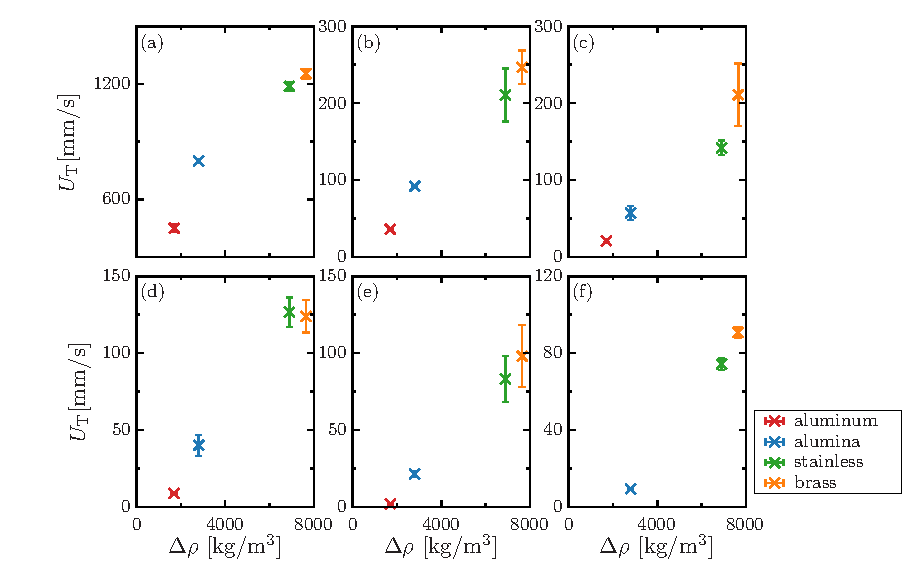
\includegraphics[width=0.9\textwidth]{./5-Results/rhoUT.eps}
    \caption{Terminal velocity with varying density difference in PAA solution (a)0.2wt.\%, (b)0.5wt.\%, (c)0.7wt.\%, (d)1.0wt.\%, (e)1.3wt.\%, (f)1.5wt.\%.}
    \label{fig:rhoUT}
\end{figure}

\begin{figure}[ht]
    \centering
    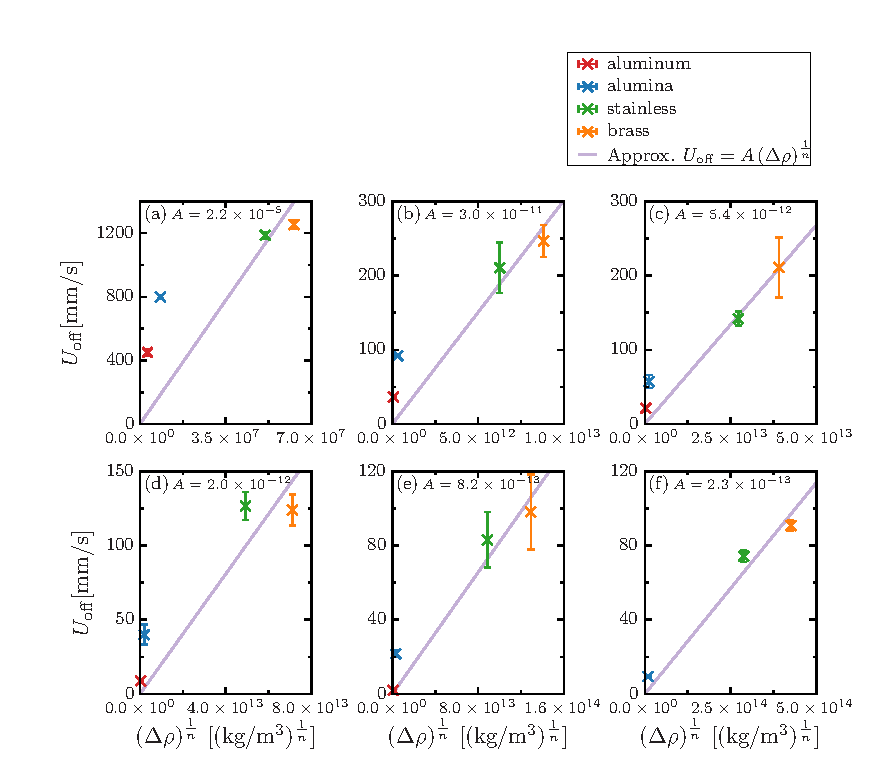
\includegraphics[width=0.9\textwidth]{./5-Results/rhoUT_index_n.eps}
    \caption{Terminal velocity with varying density difference by index $n$ in PAA solution (a)0.2wt.\%, (b)0.5wt.\%, (c)0.7wt.\%, (d)1.0wt.\%, (e)1.3wt.\%, (f)1.5wt.\%.}
    \label{fig:rhoUT_n}
\end{figure}

\begin{figure}[ht]
    \centering
    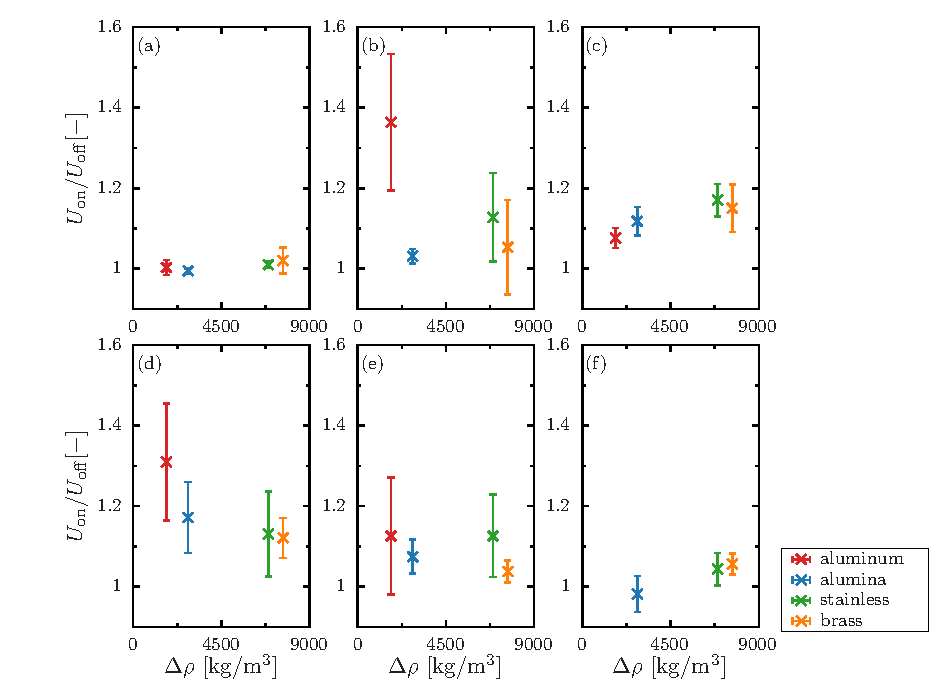
\includegraphics[width=0.9\textwidth]{./5-Results/rhoUdiff.eps}
    \caption{Velocity ratio versus density difference in PAA solution (a)0.2wt.\%, (b)0.5wt.\%, (c)0.7wt.\%, (d)1.0wt.\%, (e)1.3wt.\%, (f)1.5wt.\%.}
    \label{fig:rhoUdiff}
\end{figure}

\begin{figure}[ht]
    \centering
    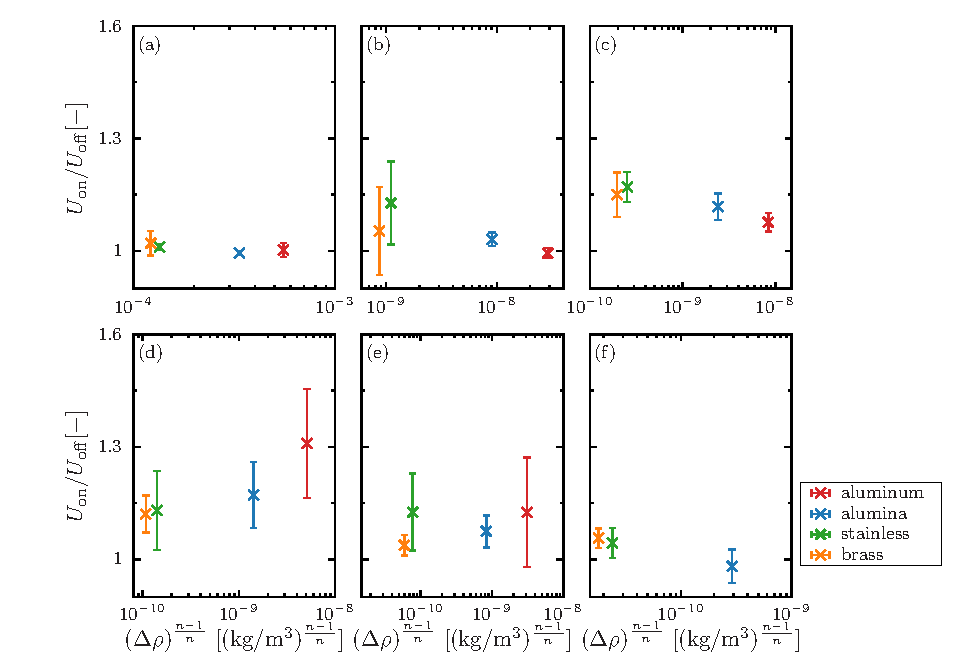
\includegraphics[width=0.9\textwidth]{./5-Results/rhoUdiff_index_n.eps}
    \caption{Velocity ratio versus density difference by index $n$ in PAA solution (a)0.2wt.\%, (b)0.5wt.\%, (c)0.7wt.\%, (d)1.0wt.\%, (e)1.3wt.\%, (f)1.5wt.\%.}
    \label{fig:rhoUdiff_n}
\end{figure}
